\section{一维核磁}
\subsection{磁自旋动量、磁矩和磁矩的能量}

在非相对论量子力学框架下,自旋的行为是通过类比角动量的行为来定义的(在学到了量子力学里可以推导),磁自旋动量$M_s$与自旋量子数$S$之间的关系(当考虑电子自旋时,自旋量子数为单电子数$n$的$\frac{1}{2}$):
\[\hat{J}^2 \varPsi = M_l^2 \varPsi \qquad M_s=\sqrt{l(l+1)} \hbar \qquad\]
\[\hat{S}^2 \varPsi = M_s^2 \varPsi \qquad M_s=\sqrt{S(S+1)} \hbar \qquad\]

磁自旋动量是一个高维向量,我们并不方便直接去研究其性质,但是我们可以在$\mathbb{R}^3$空间中研究其投影$m_{s_z}$,我们知道磁自旋动量的投影是空间量子化的,每个自旋量子数对应一不同磁自旋动量在空间上的量子化投影,共计$2S+1$个:
\[\hat{S_z} \varPsi =m_s \hbar \varPsi \qquad M_{s_z}:=m_s \hbar \qquad (m_s=-S,-S+1,...,S-1,S)\]

经典力学中带电的旋转体具有磁矩,这点在量子力学中直接被沿用,粒子自旋的磁矩$\mu$平行且正比于自旋角动量$M_{s_z}$,比例系数为磁旋比$\gamma$,这里给出磁矩和磁自旋动量的关系式:
\[\mu=\gamma M_s=\gamma \sqrt{S(S+1)} \hbar= g_N \sqrt{S(S+1)}  \mu_N\]

我们这里统一规定磁场方向为z轴正向,磁矩的同样也是一个高维向量,其投影同样也是空间量子化的,因此我们对磁矩$\mu$做$\mathbb{R}^3$空间的投影:
\[\mu_z=\gamma M_{s_z}=\gamma m_s \hbar \qquad (m_s=-S,-S+1,...,S-1,S)\]

则磁矩在磁场中的势能可以写成:
\[E=-\mu \cdot B_0=-\mu_zB_0=-\gamma m_s \hbar B_0 \qquad  (m_s=-S,-S+1,...,S-1,S)\]

由于核自旋能级跃迁的选律为$\Delta m= \pm 1$,以氢核为例,其$m_s= \pm \frac{1}{2}$,则使其跃迁即发生核磁共振现象的光子频率应为:
\[\nu_0 = \frac{\Delta E}{h}=\frac{\gamma \hbar B_0}{h}=\frac{\gamma B_0}{2\pi} \tag{a}\]

\begin{center}
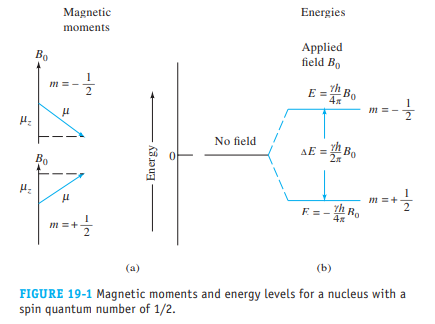
\includegraphics[scale=0.8]{./fig/hc/hc1.png}
\end{center}

\subsection{磁场下的核自旋能级}

核磁得到的数据是一组多次长时间(相对于瞬时而言)累计的信号,因此不同核自旋能级上的离子分部大致满足玻尔兹曼分布:
\[\rho_i=\frac{e^{-\frac{E_i}{kT}}}{Q} \qquad Q=\sum_{i=1}^{2S+1}e^{-\frac{E_i}{kT}} \tag{b}\]

由玻尔兹曼分布可知,与$B_0$同向的核自旋动量对应的进动圆锥面上分布这更多的粒子,不同核自旋动量对应的进动圆锥面上分布着不同数目的粒子。

\subsection{化学位移}

根据(a)式,我们可以关联起磁场与核自旋能差,但实际上,因为原子核并不会单独存在以及原子核并不是在任何情况下均不会发生变化的,分子中的电子云以及少量核自身的变化会产生一个与外加场相反的磁场抵消一部分外加场,使得\textbf{原子核感受到的磁场}并非完整的外加场,所以我们也可以定义一个屏蔽常数$\sigma$来描述这种屏蔽效应:
\[\nu =\frac{\gamma B_e}{2\pi}=\frac{\gamma (B_0-B')}{2\pi}:=\frac{\gamma B_0}{2\pi}(1-\sigma) \]

根据化学位移的定义我们可以有:
\[\delta=\frac{\nu_r-\nu_s}{\nu_s} \times 10^6=\frac{B_r-B_s}{B_s} \times 10^6=\frac{\sigma_s-\sigma_r}{1-\sigma_s} \times 10^6\]

\subsection{宏观磁矩、拉莫尔方程、核磁共振原理}

\textbf{核磁共振是一个大量分子的行为},那么我们可以知道,对于不同分子对应相同磁量子数的磁矩在空间上的分布应该是均匀的,如果我们把这些磁矩包起来,我们可以得到一个圆锥面,我们将这个圆锥面称之为进动圆锥面,采用这个命名这也许比较显然,因为原子核磁自旋轴向与磁矩重合,因此歪掉的磁矩在磁场会使得原子核发生进动。

由玻尔兹曼分布我们知道,粒子在不同进动圆锥面分布不均,因此,我们定义一个宏观磁矩M,其等于单位体积内所有粒子的磁矩的矢量和:
\[\overrightarrow{M}=\sum_i \overrightarrow{\mu}\]

定义单位体积磁矩而非整体磁矩主要的考虑是,为保证核磁能源源不断产生信号,粒子核自旋分布必须时刻保持近玻尔兹曼分布,即朝上的自旋始终多于朝下的自旋,因此整体核自旋方向应保持近平行于z轴,所以我们选取给出信号后被激发的部分或者所有粒子为一个整体做为对象。

对其进行正交分解得到沿着磁场方向的矢量和垂直磁场方向的矢量:
\[\overrightarrow{M}=\overrightarrow{M_{par}}+\overrightarrow{M_{prep}} \]

当无外加信号场时,$\overrightarrow{M_{perp}} \approx 0$,此时认为仅有沿磁场方向的$\overrightarrow{M_{par}}$,显然$\overrightarrow{M_{par}}>0$,记此时的$\overrightarrow{M_{par}}$为$\overrightarrow{M_0}$。

当未发生核磁共振的时候,在外加场的作用下,核自旋运动会产生核的进动(联想歪掉的陀螺),核自旋轴(单个核磁矩)进动围绕着z轴(磁力线),其进动的角速度和磁场有以下关系(虽然线性外加场下单个磁矩是歪的,但宏观磁矩依然是沿z轴正方向的):
\[\omega=\gamma B \tag{c}\]

此关系成为拉莫尔方程,这种进动也称之为拉莫尔进动。所谓核磁共振也就是\textbf{外加场在与某种拉莫尔进动同频的情况下为该拉莫尔进动提供能量}。下面我们来证明这个方程:

简单证明:

在外加场$B_0$存在时,核自旋进动的频率为:
\[\nu = \frac{\gamma B}{2 \pi}\]

故进动的角速度为:
\[\omega = 2 \pi \nu =2 \pi \cdot \frac{\gamma B}{2 \pi}= \gamma B\]

或者我们可以再严谨一点:

在均匀磁场$B$中,每单位体积磁矩所受力矩$M$为:

\[M=\mu \times B\]

于是根据角动量定理,得:

\[\frac{\mathrm{dL}}{\mathrm{d}t}=-M=-\mu \times B=-\gamma L \times B=\omega \times L\]

故:

\[\omega=-\gamma B\]

更进一步,我们甚至还能算出磁旋比$\gamma$,假定样品质点比荷都是$e/m$,把物体划分为许多体积元$d\tau$,则每个体积元的质量与电荷可表示为$de=\frac{e}{m}dm$,以$v$表示该体积元的速度,则电流密度$j$可表示为$j=v\frac{e}{m}\frac{dm}{d\tau}$,于是磁矩:

\[\mu=\frac{1}{2}\int r \times j d\tau=\frac{1}{2}\int r \times v\frac{e}{m}\frac{dm}{d\tau} d\tau=\frac{1}{2}\int r \times v\frac{e}{m}dm=\frac{e}{2m}\int r \times v dm=\frac{e}{2m}L\]

故磁旋比$\gamma$:

\[\gamma=\frac{e}{2m}\]

\begin{center}
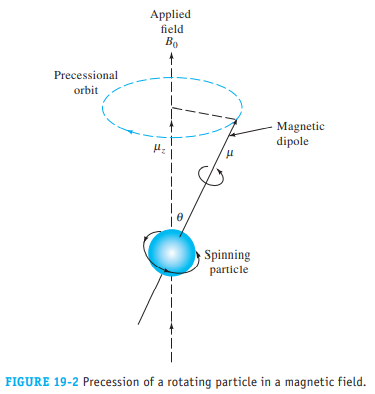
\includegraphics[scale=0.6]{./fig/hc/hc2.png}
\end{center}

拉莫尔方程告诉我们,带电体(这里是核自旋)在外磁场的存在下会绕外磁场进动,自然而然,我们可以知道宏观磁矩也会绕外磁场进动,在不发生核磁共振时外加场与宏观磁矩重合,可以认为宏观磁矩“零距离”绕磁场进动,这件事意味着我们只需要讨论磁场的取向就能较好地表述核磁共振。

这里给个例子,我们在三维直角坐标系里xOy平面上给定两个单位圆并记其上的一条半径分别为a、b,标记半径为a的圆以角速度$\omega$顺时针转动,标记半径为b的圆也以角速度$\omega$逆时针转动,两圆均以速度$v$朝z轴正方向运动,刚开始时a、b均与x轴正半轴重合。设半径a、b与圆周交点分别为A$(x_1,y_1,vt)$、B$(x_2,y_2,vt)$,可以写出A、B两点带时间参数的坐标:
\[A=(cos(\omega t),-sin(\omega t),vt) \qquad B=(cos(\omega t),sin(\omega t),vt)\]

考虑A、B中点O,则可以写出O点带时间参数的坐标:
\[O=(cos(\omega t),0,vt)\]

这时,我们会发现O点在曲线$x=cos(\frac{\omega z}{v})$上运动,这意味着我们用两个运动速度相同方向相反的圆偏振合成出了交变线偏振,当然同样的我们也可以将线性交变线偏振拆成两个方向相反的圆偏振。

因为磁场也是一种电磁波,有了上面的例子,我们可以知道:给原子核加上一个线偏振磁场相当于给原子核加上两个角速度方向相反、大小与某磁自旋量子数对应进动相同、垂直于原外加场的圆偏振磁场:
\[\overrightarrow{B}=\overrightarrow{B_0}+\overrightarrow{B'}=\overrightarrow{B_0}+\overrightarrow{B_{perp}}+\overrightarrow{-B_{perp}}\]

因为与进动方向相反的圆偏振磁场与进动在时域上正交,所有其对宏观磁矩的进动是没有贡献的,因此,我们可以给出对宏观磁矩的有效磁场$B_e$:
\[\overrightarrow{B_e}=\overrightarrow{B_0}+\overrightarrow{B_{perp}}\]

在实验室坐标系O-xyz下,宏观磁矩在旋转,磁场$\overrightarrow{B_{perp}}$也在旋转,当然我们也可以选定一个绕z轴旋转的坐标系固定磁场和宏观磁矩。所以在旋转坐标系O-x'y'z'中对宏观磁矩的有效磁场$B_e$在该坐标系下表达式为:
\[\overrightarrow{B_e}=\overrightarrow{B_0}+\overrightarrow{B_{perp}}+\overrightarrow{\frac{\omega}{\gamma}} \tag{d}\]

在旋转坐标系O-x'y'z'中$\overrightarrow{B_{perp}}$是固定的,便于处理,这也是为什么我们选择旋转坐标系的原因,这里,我们不妨将$\overrightarrow{B_{perp}}$固定在x'轴正方向。

共振时$\omega=\omega_0=2\pi \nu_0 \ , \ \overrightarrow{B_0}+\overrightarrow{\frac{\omega}{\gamma}}=0$,则有:
\[\overrightarrow{B_e}=\overrightarrow{B_{perp}} \tag{e}\]

不共振时,我们也能改写上式为:
\[\overrightarrow{B_e}=\overrightarrow{B_0}+\overrightarrow{\frac{\omega}{\gamma}}+\overrightarrow{B_{perp}}=\overrightarrow{\frac{\omega_0+\omega}{\gamma}}+\overrightarrow{B_{perp}}\]

其中$\omega_0$与$B_0$同向,$\omega$与$B_0$反向。

根据上面的讨论,我们知道,当发生核磁共振时,在旋转坐标系O-x'y'z'中,宏观磁矩$M$绕着x'轴转动,也就是发生从z'轴正方向到y'轴的偏转,其垂直外加场$B_0$的分量$M_{perp} \neq 0$,当撤去外加场$B'$,歪掉的宏观磁矩$M$会通过弛豫过程回复到原先方向。在实验室坐标系O-xyz下,在这个回复的过程中宏观磁矩$M$依旧在旋转,依然会继续切割外加场$B_0$产生信号直至其垂直外加场$B_0$的分量$M_{perp}=0$。通过检测弛豫信号,我们可以去推断这个原子核的自旋情况及其外部电子云的分布,当然对这个时域上的弛豫信号我们可以对其傅里叶变换研究其频域谱,这也就是我们常见的一维谱。

\subsection{弛豫过程}

我们都知道每一张核磁谱都是多次信号累加平均后得到的,这就意味着每次激发后激发态的原子需要回复到基态,我们把恢复到基态的这个过程称之为弛豫(relaxation)。从直观上来说,弛豫过程就是将倾斜的宏观磁矩扶正,我们有两个过程实现这个过程:

\qquad 1、将$M_{par}$的数值回复到$M_0$;

\qquad 2、将$M_{perp}$的数值减小至0;

第一种过程称为纵向弛豫,又称自旋-晶格耦合(spin-lattice relaxation),这里的晶格指的是环境,第二种过程称为横向弛豫。

对于纵向弛豫,核磁共振时,宏观矢量$\overrightarrow{M}$倾倒,$B_e$沿外加场分量变小,核自旋跃迁的能隙也变小,由于激发未饱和,基态的分子数多与激发态的分子数,能隙的变小意味着分子从磁场中吸收能量,这与核磁共振现象的描述是自洽的。纵向弛豫这是上述过程的逆过程——宏观矢量$\overrightarrow{M}$回正,$B_e$沿外加场分量变大,核自旋跃迁的能隙也变大,分子向磁场中释放能量。

对于横向弛豫,核磁共振的激发使得宏观矢量分量$\overrightarrow{M_{perp}}$不再为0,在横向上磁场分布不再均匀,这时,分子通过横向弛豫回复宏观矢量的过程是熵驱动的,分子本身不均匀的磁矩也有一定的贡献。

一般来说,纵向弛豫的耗时会大于等于横向弛豫。

\begin{center}
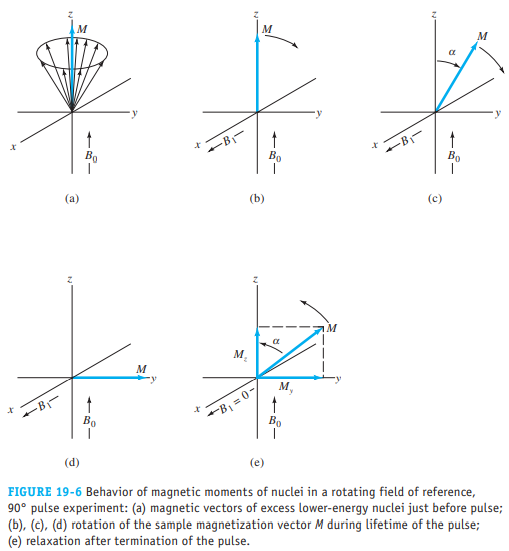
\includegraphics[scale=0.7]{./fig/hc/hc3.png}
\end{center}

\subsection{核磁共振谱的宽度}

依据海森堡测不准原理,我们有以下结论:
\[\Delta E \Delta t \sim h \tag{f}\]

(f)式中,t为横向弛豫用时。
\[\Delta \nu = \frac{\Delta E}{h} \sim \frac{1}{\Delta t} \tag{g}\]

\subsection{脉冲-傅里叶变换核磁共振}

我们知道,有效磁场$\overrightarrow{B_e}$的大小为:
\[|\overrightarrow{B_e}|=\frac{1}{\gamma}\sqrt{(\omega_0-\omega)^2+(\gamma B_{perp})^2}\]

当满足条件$(\gamma B_{perp})^2 \gg (\omega_0-\omega)^2$时,我们可以得到:
\[|\overrightarrow{B_e}| \approx |\overrightarrow{B_{perp}}|\]

这意味着当$\overrightarrow{B_{perp}}$足够大时,一定范围内所有的原子都能发生共振,不需要连续进行扫场或者扫频,打谱时间大大缩短(保证信噪比$\frac{S}{N} \propto \sqrt{n}$足够大),当然这也意味着需要使用短而强的脉冲进行核磁共振。

脉冲-傅里叶变换核磁共振具有以下优点:

\qquad 1、不论同种原子同位素处于分子何处、何种官能团上,都能同时共振;

\qquad 2、用时短,一次测量大概在微秒量级;

\qquad 3、分时装置,接受装置在发射装置后;

\qquad 4、可以使用不同种类的脉冲。

前三点保证了脉冲-傅里叶变换核磁共振用量少、用时短的优点,后两点则使得脉冲-傅里叶变换核磁共振可以完成许多CW(连续波)仪器做不到的事,比如开辟了二维核磁甚至多维核磁的利用。

\section{Nuclear Overhauser effect}

对分子中空间相距比较近(<5 \AA)的两核之一经行辐照,使之达到跃迁的饱和状态,此时记录另一和的核磁共振峰,可发现无此照射时的谱峰强度有所变化,这即使NOE效应,两个核在空间内足够接近是NOE效应的必要条件。

在以谱学方法研究立体化学时核磁共振是最有力的工具,以核磁共振研究立体化学时有以下几种方法:化学位移$\delta$值的变化、耦合常数J(与二面角$\phi$的关系)、NOE等。其中NOE是最有效的方法。

NOE产生的机制是磁性核之间的偶极耦合(dipole coupling),而通过化学键相连的磁性核的自旋-自旋耦合称为标量耦合(scalar coupling),磁性核有磁矩,磁矩与磁矩之间的相互作用正比于$\frac{1}{r^6}$,这也是为什么当两核空间上充分接近时才会有较强的NOE效应的重要原因。

\section{二维核磁}

在一维核磁的部分中,我们知道样品中的磁性核(有磁矩的核)在静电场$B_0$的作用下产生了宏观磁化矢量(宏观磁矩),为使核磁共振发生,需要一个频率恰当的电磁波。射频电磁波是线偏振磁场,可以分解为两个旋转方向相反的圆偏振磁场。其中之一与原子核进动方向相同,该旋转磁场与宏观磁化矢量$M$有相互作用。采用旋转坐标系,旋转坐标系中的旋转磁场$B_{perp}$是相对静止的,沿着x'轴正方向。$M$在$B_{perp}$的作用下,绕着x'轴转动,偏离z轴,产生了横向磁化矢量$M_{perp}$。

当我们使用合适的脉冲,我们可以将宏观磁矩旋转$90^{\circ}$至y'轴上,这样做的好处是宏观磁矩的垂直磁场分量达到最大,在检测信号时更加明显,同时这样也方便检测横向弛豫时间。由于分子内各个方向的磁矩不相同,总有一部分分子运动得快,另一部分分子运动的慢,在绕着磁场进动时,所有分子不都以角速度$2 \pi \nu$转动,但所有宏观磁矩都以$2 \pi \nu$为对称轴在一定角速度内均匀分布,这样的差异将称为我们分析分子中不同精细结构的重要信息。如何利用这些信息,将涉及到\textbf{自旋回波}的内容。

\subsection{自旋回波及其脉冲序列}

首先给出自旋回波的脉冲序列:
\[90^{\circ}_{x'}-DE-180^{\circ}_{x'}-DE, \ AQT\]

接下来我们将分3种情况讨论自旋回波并介绍一些特殊的自旋模式:

\subsubsection{无耦合时的自旋回波}

当施加一个脉冲使得宏观磁矩绕x'轴转$90^{\circ}$到y'轴上后,给其一段时间让其在实验室坐标系下绕z轴旋转,由上部分内容可知,我们设转得最快的宏观磁矩为F、最慢的为S,当施加一个脉冲使得宏观磁矩绕x'轴转$180^{\circ}$到x'Oy'平面y'负半轴区域后,S、F两者位置反转,下一个DE即为第一个DE的逆过程,在DE的最后时刻S、F都重合于y的负半轴。这样对称的过程可以\textbf{消除由于外磁场不均匀带来的误差}。同样的,自旋回波还能使\textbf{化学位移不同的同位素核化学位移重新聚集,这点在后面两种情况依然成立}。

我们可以优化一下这个脉冲序列:
\[90^{\circ}_{x'}-DE-180^{\circ}_{y'}-DE, \ AQT\]

这个优化后的脉冲序列原理于原先的基本一直,但其优势在于经过偶数次DE后宏观磁矩都在y'轴正方向上。我们都知道脉冲让宏观磁矩偏转的角度$\theta$由脉冲作用的宽度(时间)$t_p$调制,但实验中$t_p$不能完全准确,实际的脉冲角度应该为$180 \pm \theta'$,所以,经过偶数次的DE,我们可以消除这一误差来源。

\subsubsection{异核耦合体系的自旋回波} 

异核耦合体系AX的自旋回波基本于无耦合时类似,方便起见,我们只讨论其中的一个原子,对两个不同种的原子核其共振频率相差极大。

假设另外一个核对该原子核的耦合常数为$J$,我们只需将无耦合时的F换成$2 \pi \nu + \frac{J}{2}$,S换成$2\pi \nu - \frac{J}{2}$即可。同样的我们也可以发现自旋回波能将同种原子的不同耦合裂分峰重新聚焦。

\subsubsection{同核耦合体系的自旋回波} 

与异核耦合体系不同,同核体系AA两者的核磁共振频率很相近,这就使得同核耦合体系的自旋回波与异核耦合体系的自旋回波有不同,直接给结论:\textbf{同核耦合体系在经过一个自旋回波过程后,两宏观磁矩的垂直分量关于y'轴负半轴堆成,且均与之成角$2 \pi J \cdot DE$。}因为核磁共振信号强度为$\overrightarrow{B_{perp}}$在y'轴上的投影,所以在此条件下,核磁共振信号强度被$cos(2 \pi J \cdot DE)$调制(modulated),而与化学位移无关,这是后面讨论同核J谱的基础,就这样,我们开始一步步接近核磁共振二维谱了。

\subsubsection{核磁信号的相位被化学位移所调制} 

对异核体系AX,其中A为采集核,X为非采集核,我们讨论以下脉冲序列:
\[90^{\circ}_{x',A}-DE-180^{\circ}_{X}-DE, \ AQT\]

脉冲序列中$180^{\circ}$的脉冲仅作用在非采集核上,绕x'轴和绕y'轴作用类似。

到第一个DE为止都与之前的情况类似,在对非采集核的$180^{\circ}_{X}$后,$2 \pi \nu + \frac{J}{2}$与$2 \pi \nu - \frac{J}{2}$的位置互换,再经过一个DE,两者重新聚合,这时,核磁共振信号强度将被$cos(2 \pi \nu \cdot DE)$调制,即被化学位移调制,而与耦合常数无关。这时讨论异核位移相关谱的基础。

\subsubsection{BIRD脉冲序列} 

BIRD是bilinear rotational decoupling的缩写,译作双线性去耦合。其脉冲序列如下所示:

\[^1H: \qquad 90^{\circ}_{x'}-DE-180^{\circ}_{x'}-DE-90^{\circ}_{x'}, \ AQT\]
\[^{13}C: \qquad \qquad  \qquad \qquad \qquad \qquad \qquad 180^{\circ}_{x'}, \ AQT\]

对$^1H$和对$^{13}C$的$180^{\circ}_{x'}$脉冲是同时加上去的,BIRD脉冲具有以下作用:

\qquad 1、区分$^{13}C-^1H$和$^{12}C-^1H$;

\qquad 2、区分与$^{13}C$直接相连的氢(与$^1J_{CH}$相关)和与$^{13}C$间接接相连的氢(与$^2J_{CH}$、$^3J_{CH}$相关);

\subsubsection{自旋锁定} 

自旋锁定(spin locking)的模型较为简单,大致为对原子核施加一个$90^{\circ}_{x'}$的脉冲使得宏观磁矩转到y'轴正方向,这时,将$\overrightarrow{B_{perp}}$转到y'轴正方向,由于磁矩与磁场重合,他们之间的力矩为0,宏观磁矩不再转动,但弛豫过程还是在发生,所以宏观磁矩的长度会逐渐减小,所以理论上自旋锁定可以用来测定横向弛豫时间。

上面是对孤立磁矩的讨论,下面我们讨论二旋体系的情形:与NOE类似,这两个宏观磁矩都被固定在y'轴上,由于空间上足够接近,两磁矩间存在相互作用,因而构成旋转坐标系下的NOE,称为ROE(rotationg frame Overhauser effect),由ROE产生的二维谱称为ROESY。

\subsubsection{等频混合}

在了解等频混合之前我们首先要了解Hartmann-Hahn匹配(matching)和交叉极化(cross
ing-polarization)

Hartmann-Hahn匹配(matching)的具体内容为:
\[^1H: \qquad 90^{circ}_{x'}-CP-decoupling\]
\[^{13}C: \qquad CP, \ AQT\]

在$^1H$通道首先应用一个$\qquad 90^{circ}_{x'}$将磁矩转到y'轴后,立即加一个磁场将其固定住,同时打开$^{13}C$通道,并调节此通道的射频功率$B_{1C}$满足:
\[\gamma_H B_{1H}=\gamma_C B_{1C} \tag{h}\]

(h)式称为Hartmann-Hahn匹配条件,在此条件下$^{13}C$核与$^1H$核交换能量:由于$^1H$核磁旋比大、丰度高,因此此条件下将检测$^{13}C$核将得到增强性质,检测$^{1}H$核则相反。两核传递能量的过程为交叉极化。

我们知道,不同官能团由于环境的不同,同种同位素的核对应的宏观磁矩旋转频率(即化学位移)$\nu_i$不同,其在旋转坐标系下的旋转频率$\Delta \nu_i:=\nu_0-\nu_i$又称为偏置频率,也不同,这意味着其感受到的相同的射频功率$B_{1_i}$不同,因此将交叉极化推广到同核体系,由于同核体系只有一个射频功率$B_{1}$,不同官能团上的同位素核有不同的偏置频率,Hartmann-Hahn匹配条件难以达到。当然我们知道如果体系越接近Hartmann-Hahn匹配条件的要求,其交叉极化传递越好。

现在考虑两$^1H$核A、X:当满足$\nu_0 \gg \nu_A \ or \ \nu_X$时,$\nu_A$、$\nu_X$可以有以下近似\footnote{Davis D G, Bax A. J Am Chem Soc, 1985,107:2820-2821}:
\[\nu_A= \nu_0 + \frac{{\Delta \nu_A}^2}{2 \nu_0} \qquad \nu_X= \nu_0 + \frac{{\Delta \nu_X}^2}{2 \nu_0}\]

因此我们可以得到:
\[\nu_A-\nu_X=\frac{{\Delta \nu_A}^2-{\Delta \nu_X}^2}{2 \nu_0}\]

当
\[\left | \frac{{\Delta \nu_A}^2-{\Delta \nu_X}^2}{2 \nu_0} \right |<|J_{AX}| \tag{i}\]

满足时:A和X之间能有效传递磁化矢量。其物理意义为:采用强自旋锁定场时,化学位移偏差的影响小于耦合作用的影响,AX体系趋向于AA'体系,即形成一个强耦合体系。对于一个大的耦合体系来说,此耦合体系的各种磁化矢量能通过耦合常数充分相互影响,此时单个自旋模式(single spin mode)已经不复存在,取而代之的是集体自旋模式(collective spin mode)。

由上可知,为实现等频混合,自旋锁定场强度要比ROE强得多。

上述讨论的等频混合是HOHAHA和TOCSY等全相关谱的基础。

\subsection{一些二维核磁谱}

\subsubsection{COSY}

又叫$^1H-^1H \ COSY$,一般反映$^3J_{HH}$耦合关系,少数情况会有长程耦合的相关峰,当$^3J$较小(二面角接近$90^{\circ}$)时可能没有相关峰。

\subsubsection{HETCORE}

又叫$^1H-^{13}C \ COSY$,对$^{13}C$采集信号,一般反映$^1J_{CH}$耦合关系,不能反映季碳,不能反映$^nJ_{CH}$耦合关系。

\subsubsection{HMQC}

又叫HSQC,$^1H-^{13}C \ COSY$,对$^{1}H$采集信号,一般反映$^1J_{CH}$耦合关系,季碳无相关峰,归属完剩下的峰为活泼氢,对于区分非等价亚甲基、解析氢谱重叠有奇效。

\subsubsection{HMBC}

类似$^1H-^{13}C \ COSY$,对$^{1}H$采集信号,一般反映$^nJ_{CH}$耦合关系。

\subsubsection{INADEQUATE}

反映$^1J_{CC}$,准对角线$\omega_1=2\omega_2$,耦合(相邻)的一对碳$\omega_1$(横着的)相同,水平等距得分布在准对角线两侧,其$\omega_2$值对应其$\delta$值。

\subsubsection{TOCSY,HOHAHA}

全相关谱,啥都有($^nJ_{HH}$)。

\subsubsection{NOESY,ROESY}

只要空间相近的两个氢原子就会出峰,与$^1H-^1H \ COSY$有相似性,NOESY主要用于生物大分子,ROESY主要用于小分子。